\section{General Operations}

\index[subject]{operations!general}
\index[subject]{general operation|see{operations}}

\subsection{Structure}

Everything that happens in Vertebra is an \operation{}.\nomenclature{operation}{Vertebra's fundamental unit of work}  Conceptually, \operations{} are the fundamental unit of \textbf{work} in Vertebra.  With the exception of some infrastructure (i.e. direct \operations{}), they are all general \operations{}.  A general operation takes place in a few phases that provide various execution guarantees.

An operation consists of the components listed in table \ref{tbl:op-parts}.

\begin{table}
	\begin{center}
		\begin{tabular}{|p{0.35\textwidth}|p{0.55\textwidth}|}
			\hline \textbf{Component} & \textbf{Description} \\
			\hline
			\hline Scope      & a string that determines the dispatch and completion requirements of the operation \\
			\hline Type       & a string that determines which operation is dispatched \\
			\hline Parameters & a mapping of parameter keys (strings) to various parameter datatypes \\
			\hline
		\end{tabular}
	\end{center}
	\caption{Operation Components}
	\label{tbl:op-parts}
\end{table}

\subsection{Operation States}

The life of an operation goes through various states, as shown in figure \ref{fig:op-states}.

\begin{itemize}
	\item \textbf{New} --- Operation has been requested but has not started.
	\item \textbf{Ack} --- Operation has been acknowledged as allowed and may be starting.
	\item \textbf{Nack} --- Operation has been denied due to security policy, operation-specific issue, due to load, or due to old discovery information.
	\item \textbf{Run} --- Operation is executing.
	\item \textbf{Done} --- Operation has finished.
	\item \textbf{Error} --- Operation has failed at an application level.
\end{itemize}

\begin{figure}
	\begin{center}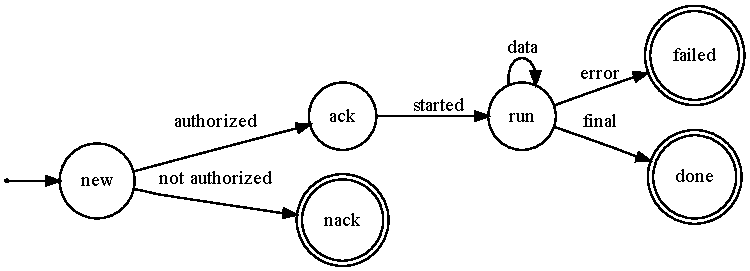
\includegraphics[width=\myfigwidth,height=\myfigheight,keepaspectratio]{figs/dot/op_states}\end{center}
	\caption{Operation States}
	\label{fig:op-states}
\end{figure}
